\chapter{Literature Review}
\label{ch:review}

The goal of this chapter is to present the research context in which our project was conducted, by looking at common methods for each of the main components and highlighting those that inspired the current approach.

In mobile robotics, map is an important prerequisite that enables robots to operate and perform different tasks such as navigation, obstacle avoidance, path planning, etc. \par \par  
\noindent Simultaneous Localization and Mapping (SLAM) is the most popular method in the literature to generate maps. Among the different methods of SLAM, vision-based and Light Detection and Ranging(LiDAR) technologies are the most popular in the literature. Although each SLAM method has its advantages and drawbacks, they are essential for different tasks. LiDAR technologies will likely remain essential for years to come due to their numerous advantages: robust to various lighting conditions, accurate 3D measurements with higher Field of View (FoV), among others, despite their high cost and bulkiness to install in small-scale robots like drones. Solid-state LiDARs are cost-effective, lightweight, and precise, making them ideal for UAVs in mapping and complex environments. 
\\ \\
Although these solid-state LiDARs have good potential, they have presented new challenges to SLAM solutions: 1) When the robot is operating in a cluttered environment, there not be strong features with geometric shapes like edges and planes. This causes the LiDAR SLAM to degenerate easily. 2) Fusing many feature points with Inertial Measurement Units (IMU) is challenging. 3) LiDAR points are sequentially sampled resulting in each point having a different timestamp which causes motion distortion that severely affects the point registration \cite{xu2021fastlio}.
\\ \\
Several works exist in the literature on LiDAR SLAM. Some of these works use filter-based (Kalman filter) approach while others use optimization-based(factor graphs) for the state estimation. Although filter-based approaches are simple in terms of implementation and computational requirements, they accumulate errors over time causing a larger drift. Optimization-based approaches on the other hand formulate the SLAM problem as non-linear problem and optimize the whole robot trajectory and the map minimizing the drift, more specifically during loop closure. Here we review the most related and relevant works.
\section{Related works}
\cite{zhang2014loam} proposed a real-time method for odometry and mapping. They achieved low-drift results without the need to use IMU and high-accuracy range measurements. The costly SLAM problem is divided into to algorithms where one algorithm computes the odometry at a higher frequency and the other algorithm runs at a much lower frequency to register point cloud.
\\ \\
A method by \cite{xu2021fastlio} presented a novel approach to tightly-coupled LiDAR-inertial odometry by proposing a new formula for computing the Kalman gain, which demonstrates equivalence to the conventional formula but reduces computation complexity based on state dimensions rather than measurement dimensions. An Iterative Kalman Filter(IKF) is used to minimize the point-to-plane distance during the registration of scan to map. The authors implemented their method into a robust LiDAR-inertial odometry package called FAST-LIO that operates effectively on a small-scale quadrotor. Experiments conducted in varied environments validate the system's resilience against fast motion and vibration noise.
\\ \\
\cite{kim2018scan} presented Scan Context, a novel spatial descriptor designed for outdoor place recognition using 3D LiDAR scans. Unlike traditional histogram-based methods, Scan Context encodes the entire point cloud into a matrix format, preserving the absolute geometrical structure of the environment. This approach utilizes a cosine distance measure for similarity scoring and implements a two-phase search algorithm to enhance loop detection efficiency, particularly in urban settings. Experimental results demonstrate that Scan Context significantly outperforms existing global descriptors in various datasets, providing robust performance against noise and viewpoint changes.

\paragraph{}  
\cite{10024300} present a novel approach for large-scale LiDAR mapping by introducing a hierarchical LiDAR bundle adjustment (HLBA) framework. The method aims to improve the consistency and accuracy of LiDAR-based maps by formulating a global optimization problem that jointly refines multiple scans. Unlike conventional SLAM techniques that rely on pairwise constraints, HLBA leverages a hierarchical structure to balance local precision and global consistency, mitigating drift accumulation over extended trajectories. The authors demonstrate the effectiveness of their approach through extensive experiments on real-world datasets, showcasing its advantages in handling large-scale environments with minimal loop closures. Their results indicate that HLBA outperforms existing methods in terms of mapping accuracy and robustness, particularly in scenarios with sparse revisits.

\paragraph{}  
A key contribution of this work is the introduction of an efficient optimization strategy that scales well with the number of LiDAR scans. By organizing the LiDAR data into hierarchical layers, the proposed framework enables efficient refinement without requiring excessive computational resources. The authors also incorporate a robust outlier rejection mechanism to enhance data association, ensuring reliable pose estimation in challenging conditions. Furthermore, the method integrates seamlessly with existing LiDAR-based odometry pipelines, making it adaptable to various robotic platforms. Overall, this study provides a significant advancement in large-scale LiDAR mapping, offering a practical solution for long-term autonomous navigation and high-fidelity 3D reconstruction.


\begin{figure}[h]
	\centering
	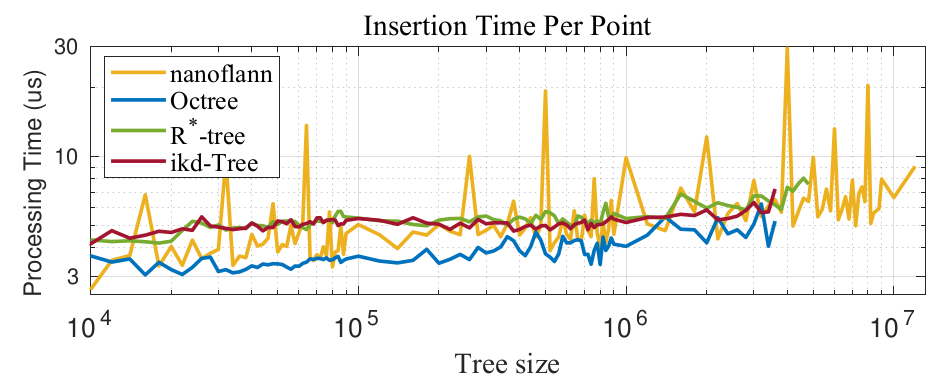
\includegraphics[width=\textwidth]{images/insert.png}
	\caption{ Insertion time per point performance of data structures for map management}
	\label{fig:insertion}
\end{figure}
\begin{figure}[ht!]
	\centering
	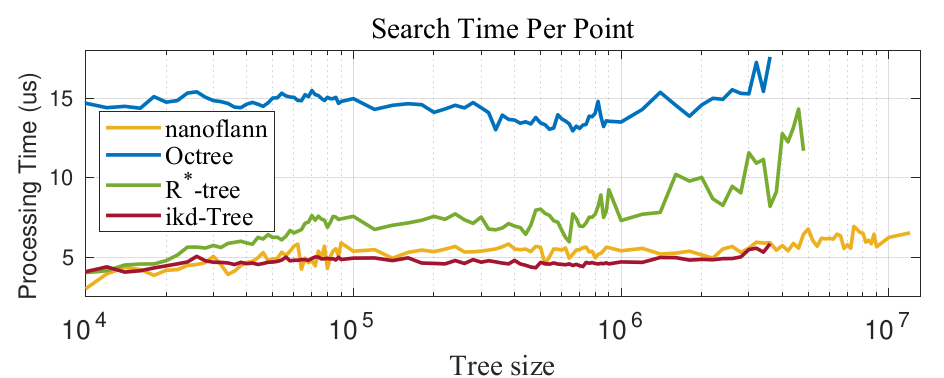
\includegraphics[width=\textwidth]{images/search.png}
	\caption{ Search time per point performance of data structures for map management}
	\label{fig:searching}
\end{figure}

\noindent \cite{xu2022fast} significantly improved upon the original work \cite{xu2021fastlio} by introducing two key advancements: direct point registration and the incremental k-D tree (\textit{ikd-Tree}). Unlike \cite{xu2021fastlio}, which relies on hand-crafted feature extraction, the new approach registers raw LiDAR points directly to the map, increasing accuracy and adaptability to different LiDAR sensors. The newly introduced ikd$\-$Tree enables efficient incremental updates, dynamic re-balancing, and on-tree downsampling, reducing computational load while maintaining real-time performance. These improvements allow a new approach to achieve higher accuracy at a lower computational cost, making it more robust for diverse environments, including those with small FoV LiDARs and aggressive motion.


As showing Figure \ref{fig:insertion} and Figure \ref{fig:searching}, ikd-Tree data structure achieves best overall performance both for point insertion time and point search time.